\chapter{An Evolutionary View on the State of the Art}\label{ch:sota}

The goal of this chapter is to survey the development of the text generation from the old days until 2020. 

As conducted from the Introduction Chapter 1, Text Generation is the generic term for the output part of an automatic text summarizer. The research on Neural Text Generation and other fields had a major impact on the development of automatic text summarizers. In this chapter, I begin with the definition of a text generator in general and its historical development. I state out the most important steps from a basic text generator to a neural text generator. In the following I focus on the text summarizer and its personal historical evolution with the impacts of the neural text generators. There are several human-like summarizing state of the art technologies nowadays for the automatic text summarizers, but they are developed under a large scale data set and computional high demanding power. I am going to mention which parts are the fundamentals for my prototype and which technologies are state of the art, but not possible to achieve with a basic home computer.

\section{The Structure of Text Generation }\label{ss:history}

Text Generation, Language modeling or Natural Language Generation are different words for basically the same meaning, but I will keep the denotation of Text Generation. A widely-cited survey from Reiter and Dale 1997 (Page 57-87) \cite{reiter} characterizes Text Generation as 'the sub-field of Artificial Intelligence and computational linguistics that is concerned with the construction of computer systems than can produce understandable texts in English or other human languages from some underlying non-linguistic representation of information' \cite{reiter}. This definition implies rather a data-to-text approach instead of the text-to-text approach from Table \ref{tab:nlp_table}, but in 1997 the rule-based approach dominated the neural end-to-end (Neural Text Generation) methods (Figure \ref{rules_based}). For that reason, in 2003 Evans declares Text Generation as quite difficult to define \cite{evans} (Page 144-151). Most researchers agree on text as the output synthesis part of the input-output system (e.g. Text Summarization or Image caption generation \cite{mitchell}). Whereas the input part can be not as easily distinguished \cite{mcdonald} (Page 191-197).

\subsection{Text Generation Tasks}

For the Text Generation input-output system, the system can be divided into six sub-problems \cite{reiter}. The following bullet points contain the six most crucial steps:

\begin{itemize}
	\item \textbf{Content determination}: Deciding which information to include in the text under construction
	\item \textbf{Text structuring}: Determining in which order information will be presented in the text
	\item \textbf{Sentence aggregation}: Deciding which information to present in individual sentences
	\item \textbf{Lexicalisation}: Finding the right words and phrases to express information
	\item \textbf{Referring expression generation}: Selecting the words and phrases to identify domain objects
	\item \textbf{Linguistic realization}: Combining all words and phrases into well-formed sentences
\end{itemize}

These six tasks can be though of an early decision processes. They suggest both a chronological order in which the tasks need to be solved, as well as an distinction between strategy and tactics. This distinction goes back to Thompson H. in 1977, where he first declared this two parts \cite{thompson}. Still, when it comes to modern neural state of the art Text Generation, the steps intersect in some ways. In the following comes a brief introduction to each of the steps. For the headline example is no aggregation necessary.

\subsubsection{Content Determination}\label{ss:content}

The first step is to determine which content should be present in the generated output text. Usually there is more information stored in the input than in the output. For this reason a certain \textit{choice} must be undertaken for the content. As mention in the case study (Section \ref{ss:case}, the headline can be summarized very precisely given only the first few sentences of the news. In this special case the determined content could be the first three sentences. For shorten a longer document into a summary, the key points need to be abstraced into a collection of preverbal messages and semantic representations of information, often expressed in the form of a logical or database like style \cite{gatt}. This means basically to group semtantical similar words and phrases together, to remove redundancies. This step followed for the most time a rule-based approach, but in recent years researchers developed a data-driven approach (more in Section \ref{ss:archi}). For example, Barzilay and Lee (2004) developed a method to determine the content through Hidden Markov Models (HMM) \cite{lee} (Pages 113-120). Hidden Markow Models are stochastical models named after the russian mathematician A. A. Markow. They chain up different states of a system, in our case different topics of one or many news articles. This topics automatically will be clustered together as sentences based on the natural language semantical meaning \cite{gatt}. 

\subsubsection{Text Structuring}

After successfully deciding which contents will be used in the generated text, the structure or order of this fragments need to be determind. Given the example article from Table \ref{tab:google}:

\begin{tcolorbox}
\begin{center}
		Australian wine exports hit a record 52.1 million liters worth 260 million dollars (143 million us) in september, the government statistics office reported on monday 
\end{center}
\end{tcolorbox}

A good news headline should give all necessary information for the reader, namely:

\begin{itemize}
	\item Where did it happen? -> \textit{Australia}
	\item What happened? -> \textit{Wine exports, record high}
	\item Who did something? -> \textit{Australia}
	\item When did it happen? -> \textit{September}
\end{itemize}

For our example the content was already predefined in the first step, now the important words and sentences will be reorder based on this four questions. Generalization approaches for the ordering task have already been proposed. Lapatas approach \cite{lapata} (Page 471-484) tries to find an optimal ordering of \textit{information-bearing-items}. This method can even be applied to multi document input, which is more difficult to solve than single document inputs (explained in Section \ref{ss:multidoc}).

\subsubsection{Sentence Aggregation}

By combining separate sentences with similar meaning into one, the generated text becomes potentially more fluid and enhances the readability \cite{dal} (Pages 383-414) \cite{cheng-mellish2000} (Pages 183-193). For example, an aggregation makes sense for a football games and its results published in the Google News. Google could web scrape the live tickers of goals and after collecting all the data a possible result would be:

\begin{tcolorbox}
	\begin{center}
		(1) Mario Götze scored after 19 minutes and 23 seconds \\
		(2) Mario Götze scored after 20 minutes and 30 seconds \\
		(3) Mario Götze scored after 60 minutes and 11 seconds
	\end{center}
\end{tcolorbox}

This is obviously not redundant, because it contains new information in every sentence, but for summarizing it, the sentences can be aggregates into:

\begin{tcolorbox}
	\begin{center}
		(4) Mario Götze scored 3 times within 51 minutes
	\end{center}
\end{tcolorbox}

Aggregation is not an easy task, because it is not intuitive for an algorithm to detect semantic similarities and at the same time new information in that. Furthermore it depends highly on the to achieving output which kind of aggregation the text should undergo. A general approach was proposed by White and Howcraft (2015). They designed an algorithm to detect parallel verb phrases (\textit{scored after}) in multiple (three) sentences and elide the subject and the verb in the generated sentence \cite{white-howcroft-2015-inducing} (Pages 28-37). 

\subsubsection{Lexicalisation}\label{ss:lex}

After the sentences have been aggregated and finalized, the next step is lexicalisation, which converts the sentences into natural language. A single event can be expressed by natural language in multiple ways. For example the scoring event from the last section could be expressed as \textit{scored three goals} or \textit{goaled for three times}. The complexity for the lexicalisation step correlates with the amount of alternative sentences available. Furthermore it is important if there summary is limited with an amount of variation \cite{Theune} (Pages 47-86). Whether or not the text shall be processed with lexical variation in its generated sentences or not depends on the application field. In needs to be decided in advance. For example the soccer game is more likely to be converted into a different styles than a weather forecast. Another important difficulty is to design the way on how the lexicalisation cares about gradable properties. For example if the liveticker was:

\begin{tcolorbox}
	\begin{center}
		(1) Mario Götze scored fast after 3 minutes and 23 seconds
	\end{center}
\end{tcolorbox}

Then the systems needs to know whether the football player scored fast in a way that it is an early stage of the game, or he ran in such a fast way and scored with the pace. Humans tend to perceive different, as Power and Williams (2014) pointed out in an evaluation. A timestamp expression of \textit{00:00} can be perceived as \textit{midnight}, \textit{late evening} or simply even \textit{evening} for some people \cite{Power} (Pages 113-134).


\subsubsection{Referring Expression}\label{ss:ref}

Referring Expression Generation is highly characterized by Dale and Reiter in 1997. They came up with the idea to identify words and phrases as domain entities. Nowadays this is also known as \textit{Named Entity Recognition}. This step shows some similarity to lexicalisation, but Dale and Reiter pointed out that expression referring is \textit{a discrimination task, where the system needs to communicate sufficient information to distinguish one domain entity from other domain entities} \cite{reiter2}. From the previous example, \textit{Mario Götze} can be denoted with his name, another way would be calling him \textit{football professional} or \textit{the athlete}. Many factors play a role in how to determine which expressions and factors play a role in a particular context. Referring expression generation can basically be broken down into two steps.
The first step is to decide the shape of referring expression. What type of reference should be used (e.g., a proper name or described with his/her job) \cite{named}. The second is to determine the content of the referring expression (e.g., Mario Götze or the athlete) \cite{named}.
Rule-based approaches as well as the state of the art Machine Learning approaches have been proposed to solve this task \cite{reiter2}.  

The usual limitation of previous referring expression generation systems is that they are not able to generate referring expressions for new, unseen entities \cite{anja} (Pages 294-327). With the use of modern Machine Learning approaches, this limitation has overcome.
Many tools, for example the \textit{Natural Language Processing Toolkit NLTK} allow the easy transformation from the lexicalized sentence into its named entities. The sentence \textit{Mario Götze scored fast after 3 minutes and 23 seconds} will be transformed into:

\begin{tcolorbox}\label{box:1}
	\begin{flushleft}
		(1) [('Mario', 'NNP'), \\
		(2) ('Götze', 'NNP'), \\
		(3) ('scored', 'VBD'),\\
		(4) ('fast', 'RB'),\\
		(5) ('after', 'IN'),\\
		(6) ('3', 'CD'),\\
		(7) ('minutes', 'NNS'), \\
		(8) ('and', 'CC'),\\
		(9) ('23', 'CD'),\\
		(10) (Seconds', 'NNS')]
	\end{flushleft}

	\begin{itemize}
		\item \textbf{NNP} = noun, proper, singular (1,2)
		\item \textbf{VBD} = verb, past tense (3)
		\item \textbf{RB} = adverb (4)
		\item \textbf{IN} = preposition or conjunction (5)
		\item \textbf{CD} = numeral, cardinal (6, 9)
		\item \textbf{NNS} = noun, common, plural (7, 10)
		\item \textbf{CC} = conjunction, coordinating (8)
	\end{itemize}
\end{tcolorbox}
\subsubsection{Linguistic Realization}

Finally after detecting all relevant words and structures of the input text, it only needs to be combined into a well-formed sentence. Usually referred to as linguistic realisation, this task involves ordering constituents of a sentence, as well as generating the correct morphological shapes (e.g verb conjugations) \cite{gatt} (Pages 18-20). The special task in this step is whether the generated output needs to make use of words not present in the given text. In the case of text summarization, this is often referred to as an \textit{abstractive} or \textit{extractive} approach (shown in Section \ref{ss:exabs}). This task can be thought of an non-isomorphic (not reservable, because the same word can have different named entities dependent on the sentence) structure \cite{ballesteros-etal-2015-data} (Pages 387-397). The three most common approaches for the realization are:

\begin{itemize}
	\item Human-crafted templates
	\item Human-crafted grammar-based systems
	\item Statistical approaches
\end{itemize}

The most modern and widely used way is the statistical approach, but within that, there are several different methods to make us of the statistics. Just to give an example, Bohnet et al. (2010) \cite{bohnet-etal-2010-broad} (Pages 98-106) describe a realizer with underspecified dependency structures as input, Support Vector Machine (SVM) based environment. The classifiers are organised in a cascade to decode semantic input into the corresponding syntactic features. A Support Vector Machine is an algorithm to classify input whether it belongs to a specific topic or e.g. named entity from the last section or not. This can also be referred to as being a \textbf{Deep Learning} approach and it was applied on a common metric for measuring the accuracy of a generated e.g. text summarization called BLEU. This metric will be explained in Section \ref{ss:ev}. Furthermore, the more decision the statistical generating system makes and the more complex it becomes, the more abstract will the output be \cite{gall} (Page 21). This paves the way for an stochastical end-to-end system, like Konstas and Lapata showed in 2013 \cite{Konstas:Lapata:2013}. This presents a step words the automated text summarizations.

\subsection{Architectures and Approaches}\label{ss:archi}

After the overview of the six main tasks for Text Generation systems, this section focuses on the way those tasks can be organized together. There are three main approaches for the Text Generation architecture shown in the dark boxes in Figure \ref{architecture}. The light boxes illustrate the outputs from the main stages.

\begin{figure}
	\begin{center}
		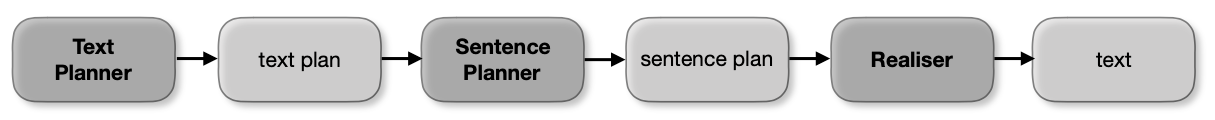
\includegraphics[width=6in]{photos/architecture}\\
		\caption{Classical 3-stage Text Generation architecture, after Reiter and Dale (2000) \cite{reiter2} }\label{architecture}
	\end{center}
\end{figure}

Since the design of the modules in Figure \ref{architecture}, a lot has changed. The modular view is challenged by the planning-based and data-driven approach, because the modular view is not flexible enough for modern requirements, still it provides a good sequence structure and the original idea remains until now. The following three approaches will be explained in more detail in this section:

\begin{itemize}
	\item Rule-based, modular approaches
	\item Planning-based approaches
	\item Data-driven approaches
\end{itemize}

\subsubsection{Rule-based approach}\label{ss:rule}

The rule-based, or modular approach shown in Figure \ref{architecture}, is a classical approach from the early Artificial Intelligence research. It is designed to show a clear division between the sub-tasks, but with sometimes big variations among them. The three-stage architecture was originally called \textit{consensius pipeline}, because the it is in the design of a pipeline and it was the de-facto standard in the year 2000 \cite{reiter2}. This pipeline share many similarities with the state of the art architecture used for text summarization in the year 2001 introduced by Mani et. al. \cite{mani}. It can be broken down into the following steps \cite{gatt} (Page 23):

\begin{itemize}
	\item \textbf{Analysis} of the source text (single or multi document). This first stage includes \textit{Text Planning}, which shares similar aspects with the Text Planner from Figure \ref{architecture}. One of the tasks for this step is \textit{Content Determination}.
	\item \textbf{Transformation} of the selected input. This phase includes processing steps like \textit{Text Structuring} and \textit{Text Aggregation} on the selected text. It is especially important when it comes to abstractive text summarization (Section \ref{ss:exabs}). This phase shares a number of similarities to the \textit{Sentence Planner} from Figure \ref{architecture}.
	\item \textbf{Synthesis} produces the summary of the input based on the transformed selected input. The higher the abstraction level of the output should be, the more important is this phase. It can be seen as the \textit{Realiser} with the methods of the \textit{Linguistic Realiser} from the previous section.
\end{itemize}

The strict breakdown into clear stages (modules) comes with the cost of decreased flexibility. There is not always a rule for each task and the state of the art results are achieved by abstractive based methods for Text Generation. Those alternative approaches with a better abstraction level come on the other hand with the cost of blurred boundaries in the single stages. The basic idea is to create hand-crafted templates for all possible circumstances. To keep up with the football example, a template could look like this:

\begin{tcolorbox}
	goals(
		\begin{addmargin}[1cm]{1cm}
			player-name = 'Mario Götze',\\
			minute = 19,\\
			seconds = 23,\\
			player-number = 10
		\end{addmargin}
		
	)\\
	
	foul(
		\begin{addmargin}[1cm]{1cm}
			by-player = 'Mario Götze',\\
			to-player = 'Thomas Müller',\\
			minute = '20',\\
			second = '12'
		\end{addmargin}
	)
\end{tcolorbox}

Even for a single football game it is obviously not possible to create a template with all possibilities. There may be some cases in which the possible combination of semantic units is not as big as in a single football game. In this cases a rule-based template could make sense, but for the most modern use-cases this approach is obsolete.

Even in the rule-based architectures have been many developments proposed, but for the sake of simplicity I want to discuss the modern approaches in more details than this old ones.

\subsubsection{Planning-based approach}

In the Artificial Intelligence field, the planning problem can be described as the process of detecting a sequence of one or more actions to satisfy an to achieving goal \cite{gatt} (Page 25). The classical planning-based approached was introduced by Fikes and Nilsson back in 1971 \cite{Fikes:71} (Pages 189-208). The idea was to to store actions into tuples containing of the preconditions and effects of the action respectively. In this way, planning-based means to regard language as an action \cite{clark}. 

Basically no restriction prevents the actions from choosing a type that can be inserted into a plan, plan-based approaches cut across the edges of many Natural Text Generation tasks that are normally strictly stacked in the classical pipeline architecture (Figure \ref{architecture}) \cite{gatt}. This means that the plan-based approach does not rely on the pipeline architecture, but steps are whirled together and follow different sequences than usually. This allows the input to be more flexibly processed. The most modern way for an planning-approach is the \textit{stochastical planning using Reinforcement Learning}. Reinforcement Learning means, that the algorithm has an implemented reward and punishment variable, which allows the algorithm to notice by itself when a certain action will be rewarded or punished. The reward and punishment need to manually configured. The Text Generation process could be modeled by an Long Short Term Memory (explained in Section \ref{ss:lstm}. The time transitions \textit{t} and the following \textit{t+1}, ... , are associated with a reinforcement signal, via the reward or punishement function to adjust the behaviour of the wanted output. 
	
Rieser et al. (2011) pointed out that this approach is effective in optimising information presentation when generating restaurant recommendations \cite{rieser}. Janarthanam and Lemon (2014) applied this method to improve the choice of information for selecting in a referring expression, given the knowledge of the user.  As the user acquires new knowledge in the course of a dialogue, the system learned to adapt its behaviour by changing its internal user-model \cite{janarthanam-lemon-2014-adaptive} (Pages 883-920).

\subsubsection{Data-driven approach}\label{ss:data}

Data-driven models experience recently more and more attention in the Text Generation community. They provide the flexibility and potential to overcome the templates based approaches. Even in the past six years, there have been plenty of studies which show the successes of data-driven models. For example on Dinu and Baroni (2014) recommend that the Text Generation can be performed by using different distributional semantic models \cite{dinu-baroni-2014-make} (Pages 624–633). Another example is from Swanson in 2014 as well, where he performed Text Generation with language modeling on a specified vocabulary constraint \cite{swanson-etal-2014-natural} (Page 124). All of this methods and data-driven approaches in general require a lot of training data. The first step in general for such system is to build up an so-called \textit{corpus}. A corpus can be viewed as a kind of template as well, but the way it is used is completely different. The corpus is created through the training of a huge training data set. It consists of a basic set of utterances and it can be further manually extended and redefined \cite{elena} (Page 4). The data-driven model can even be used for a general purpose Machine Translation system, which can respectively even be adapted to a specific domain itself (shown by Wang et al. \cite{wang-hirst-2009-extracting} Pages 471–477). The corpus contains now a set of vocabulary which can be extended through adding new training instances (e.g. user inputs or synonyms) into the \textit{lexicon}. 
Extending and diversifying the corpus enhances the quality of the interaction between
the system and the user and further enriches the conversational level, mostly the systems response. This can be regarded as a higher abstraction level, used for the modern text summarization systems. 

It can be seen in Figure \ref{corpus}, that the there is a total amount of 34283 words in the English part of the TownInfo corpus and that there are only 462 distinct tokens. This includes even varied units as proper names and numerals. This example shows an approach to translate from English into French and vice versa. All of the \textit{Advanced Approaches for Text Summarization} (Section \ref{ss:trends}) are fully data-driven. For this reason I provide no more examples.

The prototype from Chapter 3 is based on a data-driven approach as well, because my text summarizer makes use of Long Short Term Memory cells. More specifically, it is an enhanced modification, namely an Attention model. This data-driven approach will be explained in the next Section \textit{Advanced Approaches for Text Generation}.

\begin{figure}
	\begin{center}
		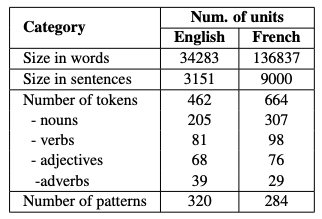
\includegraphics[width=3in]{photos/corpus}\\
		\caption{Example Corpus from \cite{elena} Page 103}\label{corpus}
	\end{center}
\end{figure}

\section{Advanced Approaches for Text Generation}
\subsection{Recurrent Neural Networks}
Even though I introduced the neuron in a neural network as a kind of brain cell imitation, the neuron of a basic neural network will forget everything when it is shut down, unlike the brain. Making information persistent is a crucial step towards better performing models. Recurrent neural networks, or RNN, address this issue. They are networks with integrated loops, which allow the information to persist \cite{olah}. The network architecture of the RNN is important, because it denotes the first step into neural text generation and neural text summarization. 

\begin{figure}
	\begin{center}
		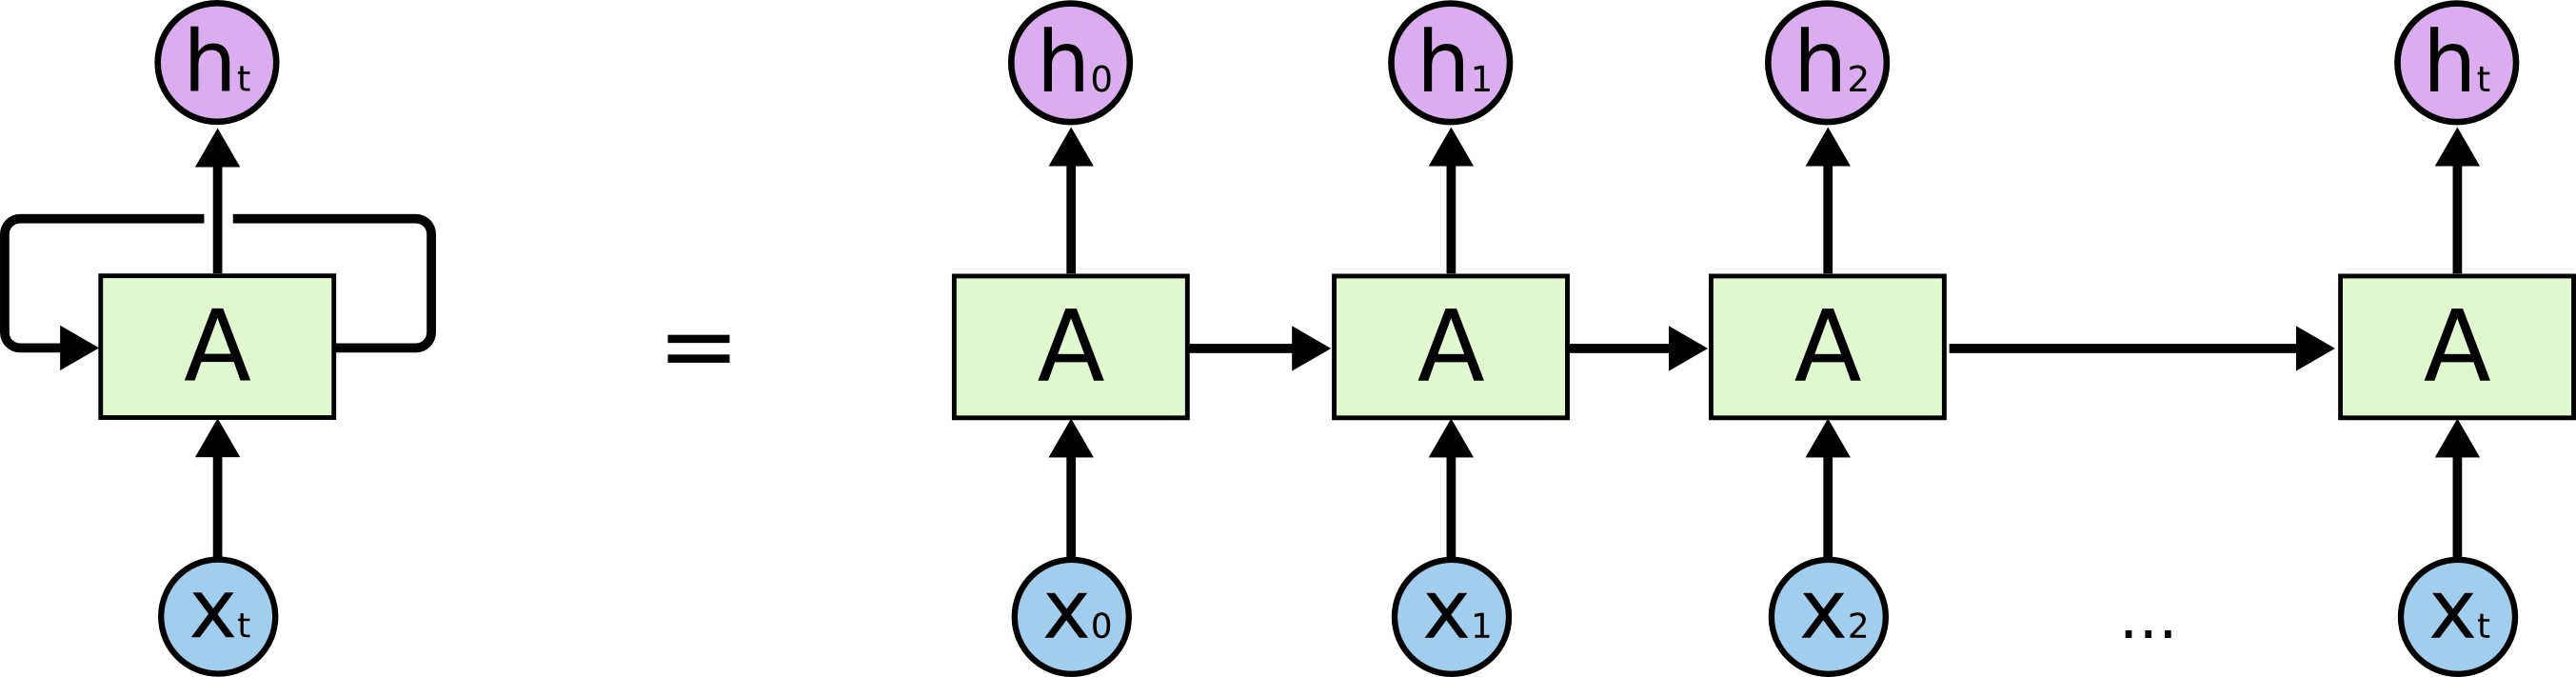
\includegraphics[width=4.5in]{photos/RNN-unrolled}\\
		\caption{Recurrent Neural Network with integrated loops \cite{olah}}\label{rnn}
	\end{center}
\end{figure}

Figure \ref{rnn} shows an unrolled Recurrent Neural Network. The input \(x_t\) on time step \textit{t}, is passed to the neural network \textit{A}. The network looks at the input on this time step and outputs the hidden state \(h_t\) at the same time step \textit{t}. This loop allows the network to pass information from one time step to another. The picture \ref{rnn} shows, that the learned parameter from input \textins{x} on time step \textins{t} will be passed as additional information to the next time step \textins{t + 1} and so on. For example if a RNN wants to predict the next word in the sentence "Since I am living in Hong Kong .. by now I speak fluent \textit{Cantonese}". The network needs to remember that the target country is Hong Kong to predict the language Cantonese. At each time step \textit{t}, the hidden state \textit{\(h_t\)} of the Recurrent Neural Network is updated by:

\begin{center}
\begin{math}
\boldsymbol{h_{(t)}} = f(\boldsymbol{h_{(t-1)}}, x_{t})
\end{math}
\end{center}

where \(f\) is a non-linear activation function and \textit{x} is the input in form of a word. The function \(f\) can be in the simplest case a sigmoid function which has either 0 or 1 as output, or the more complex and effective Long Short Term Memory cell, explained in the next Section \ref{ss:lstm} \cite{hochreiter1997long}. The Recurrent Neural Network is trained to predict for example the next word in a sentence or sequence. This prediction is possible due of the learned probability distribution over a sequence. The output at each time step \textit{t} is a conditional distribution \(p(x_{t}|x_{t-1},...,x_{1})\).

Theoretically with this approach it is possible to retain information from many time steps ago, but unfortunately, as the time span back grows, RNN's become unable to learn the information from too long ago cells. This phenomenon was explained by Sepp Hochreiter in 1991 \cite{Hochreiter:91} under the name \textit{vanishing gradient problem}. The solution to this problem is the Long Short Term Memory, short LSTM.

\subsection{Long Short Term Memory}\label{ss:lstm}
Long Short Term Memory cells were first proposed by Sepp Hochreiter and Jürgen Schmidhuber in 1997 \cite{hochreiter1997long}. The LSTM is a special kind of Recurrent Neural Network, because it is able to remember long-term dependencies and informatiom. The goal of the cell is to solve the vanishing gradient problem of the Recurrent Neural Network. Inputs into this cell can be stored for a long period of time, without forgetting them, as in Recurrent Neural Networks. The LSTM is designed to avoid the loss of information (vanishing gradient problem), by intentionally ledging on to certain information over plenty of time steps. 

\begin{figure}
	\begin{center}
		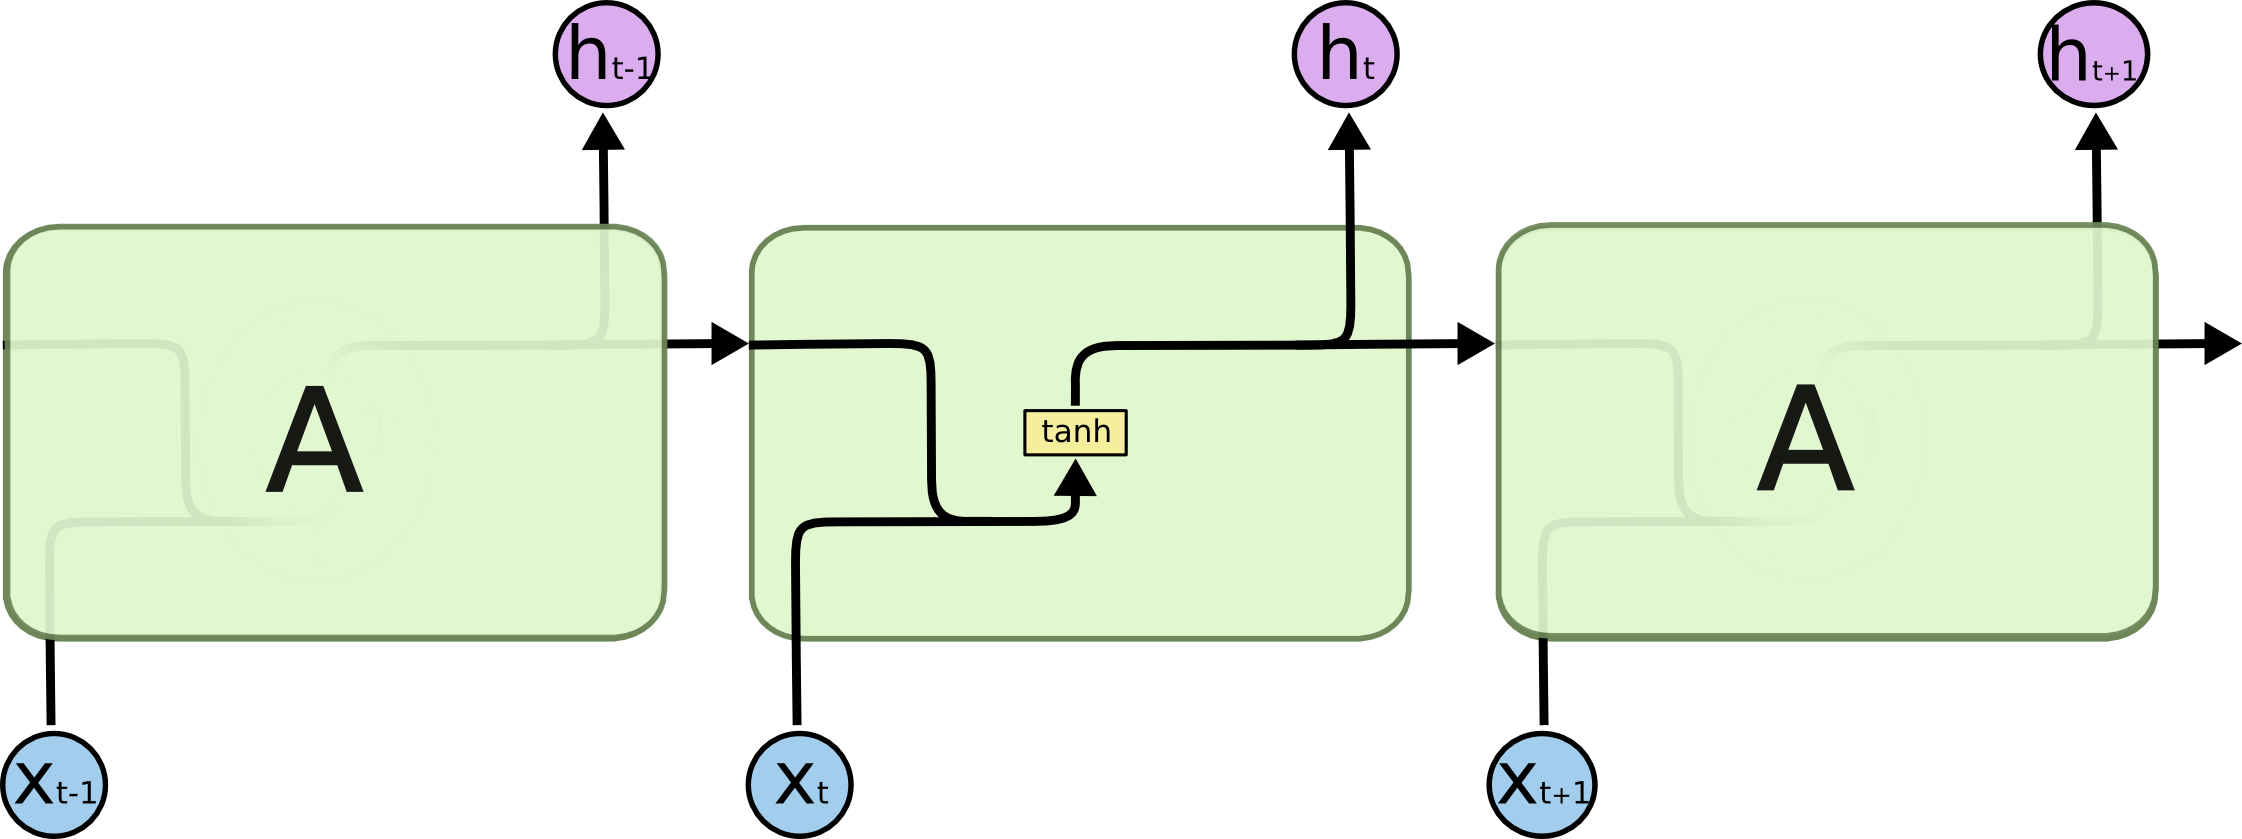
\includegraphics[width=4.5in]{photos/LSTM3-SimpleRNN}\\
		\caption{The repeating module in an Recurrent Neural Network contains one single layer \cite{olah}}\label{lstm}
	\end{center}
\end{figure}

LSTM's can be enrolled the same way like RNN's, but there is a core difference between the Recurrent Neural Network in Figure \ref{lstm} and the Long Short Term Memory in Figure \ref{lstm2}. The LSTM has four gates instead of one like the RNN. The four gates are:

\begin{itemize}		
	\item Forget Gate
	\item Input Gate
	\item Cell State
	\item Output Gate
\end{itemize}

\begin{figure}
	\begin{center}
		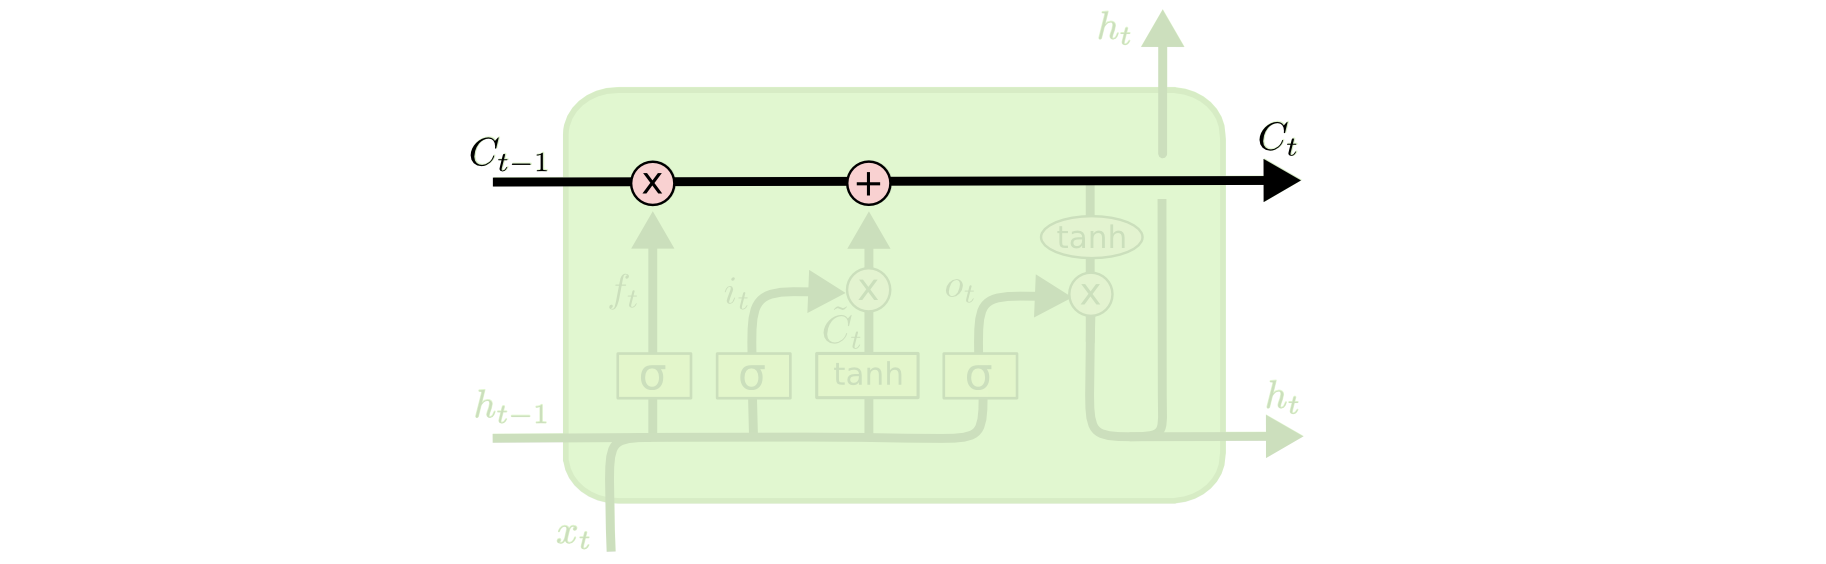
\includegraphics[width=4.5in]{photos/LSTM3-C-line}\\
		\caption{Cell State of the Long Short Term Memory which acts as data highway \cite{olah}}\label{lstm3}
	\end{center}
\end{figure}

The \textbf{Forget Gate} decides what information should be thrown away or kept. Information from the previous hidden state and information from the current input is passed through a sigmoid function. A sigmoid function takes an input and returns high values closer to 1 and smaller values closer to 0. The closer to 0 means to forget the state, and the closer to 1 means to keep the state.

The \textbf{Input Gate} updates the cell state. That decides which values will be updated by computing the values to be between 0 and 1 like the Forget Gate. Important information is closer to 1 and 0 means less important.

The \textbf{Cell State} is the core of the LSTM. It is the horizontal line shown in Figure \ref{lstm3}. The cell state acts like the information highway in the cell. With only some minor linear computation, it runs through the entire cell. This way information can pass very easily through the cell. 

The \textbf{Output Gate} decides what the hidden state of the next LSTM cell should be. The hidden state contains information on previous inputs and it is also used for predictions. The hidden state denotes the state which is passed from the output gate on time step \textit{t} to the input gate for the LSTM cell on time step \textit{t+1}.


\begin{figure}
	\begin{center}
		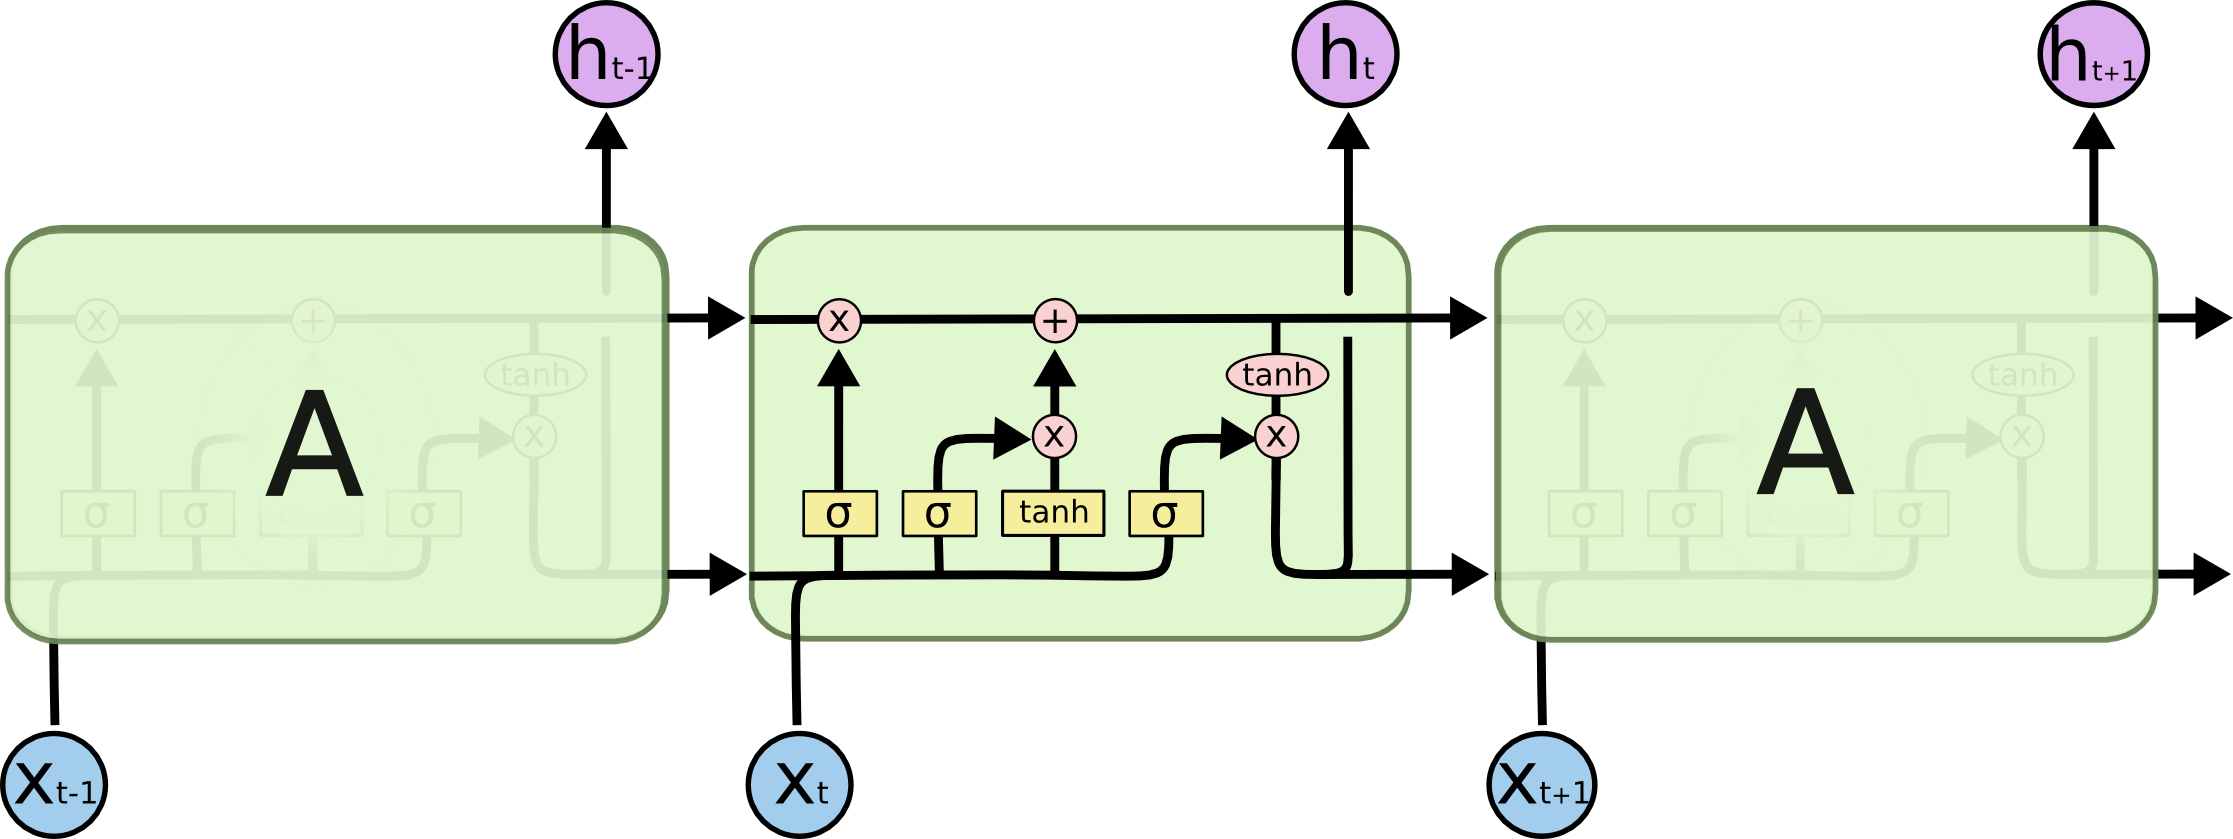
\includegraphics[width=4.5in]{photos/LSTM3-chain}\\
		\caption{The repeating module in an LSTM contains four interacting layers \cite{olah}}\label{lstm2}
	\end{center}
\end{figure}

The main idea of the LSTM is, that it can decide which information to remove, to forget, which to store and when to use it. It can also decide when to move the previous state information to the next, like the RNN shown in Figure \ref{rnn}. Even though many variations of the LSTM occupy the state of the art performance, the LSTM is used in many real business cases in production, like the Google translater or weather forecasting.
The Long Short Term Memory paved the way for the sequence to sequence models.
\subsubsection{N-Grams}\label{ss:ngram}

\subsection{Sequence to Sequence}\label{ss:seq2seq}
In the year 2014, Google invented a new way to translate language by learning a statistical model with a neural machine translation approach \cite{seq2seq}. Google called it Sequence to Sequence model \cite{seq2seq}, often shortened down to seq2seq, which consists of an encoder and a decoder. 

Before that, language translation was originally processed by rule-based systems \cite{chen-goodman}. The systems computed their work by breaking down sentences into plenty of chunks and translating them phrase-by-phrase, but this approach created not easily understandable language.

After rule-based systems, statistical models have taken over the. Given a source text in e.g. German (\textit{f}), what is the most suitable translation into e.g. English (\textit{e})? The statistical model p(\textit{g}|\textit{e}) is trained on multiple texts (corpus) and finally outputs p(\textit{e}), which is calculated only on the target corpus in English. 

\begin{center}
\begin{math}
\hat{e} = argmax_{e}(e|g) = argmax_{e} p(g|e) p(e)
\label{eq:rule}
\end{math}
\end{center}

The formula means, among all Baysian probabilities p(\textit{g}|\textit{e})p(\textit{e}), select the pair of words (translation), select the most likely to be the best translation (argmax). Even though this approach produces good results, it looses the wider semantical view, and so it is especially not effective for a good summarization technique.

For the first time, neural networks in form of feed-forward fully-connected neural networks produced such good results, that they replaced all non-network techniques. Affine matrix transformations are stacked together and are followed by non-linearities to the input and each following hidden layer \cite{Bengio} Page 1141-1142. However, these models require a fixed content length for their calculations, which makes them again not flexible enough to produce human-like translations. 

Even if a LSTM (Section \ref{ss:lstm}) was used to map sequences of words from one language to another, it will most likely produce errors or bad results. A single LSTM cell needs the same input length and output length, which is unrealistic for translating multilingual. For example the English "He is running" translated into German is "Er rennt". The LSTM itself can not translate that, because of the different word length. 
The Long Short Term Memory cell from Section \ref{ss:req} was invented independently from the sequence to sequence models, but
finally three employees of Google published a paper about their approach to make use of the LSTM to create a sequence to sequence model, also called encoder-decoder model.
The basic idea is that the encoder converts an input text to a latent vector of length \text{N} and the decoder generates an output vector of length \textit{V} by using the latent encoded vector. It is called a latent vector, because it is not accessible during the training time (manipulating it), for example in a normal Feed Forward Neural Network, the output of a hidden layer in the network can not be manipulated. The initial use of encoder-decoder models was for machine translation.

Technologies for a specific field in the machine learning environment and especially text generation can often be used cross functional. The encoder-decoder model found its way into text summarization and automated email reply by Google \cite{google} as well. Figure \ref{enc-dec} illustrates the model for Google's automated email reply.

\begin{figure}
	\begin{center}
		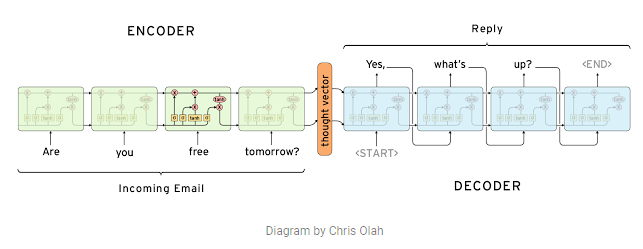
\includegraphics[width=5.5in]{photos/encoder_decoder}\\
		\caption{LSTM encoder-decoder model for automated E-Mail reply}\label{enc-dec}
	\end{center}
\end{figure}

Figure \ref{enc-dec} makes use of an Long Short Term Memory cell, which captures situations, writing styles and tones. The network generalizes more flexible and accurate than a rule-based model ever could \cite{google}. 


\subsection{Encoder and Decoder}

In the following, the encoder and then the decoder will be explained to have a better insight in how this technology works. The prototype from Chapter \ref{ch:proto} is based on this kind of model. As already mentioned a sequence to sequence model is often referred to as a encoder-decoder model. The sequence to sequence model itself is built using a Recurrent Neural Network or a Long Short Term Memory as explained in the last Section \ref{ss:seq2seq}.

\begin{figure}
	\begin{center}
		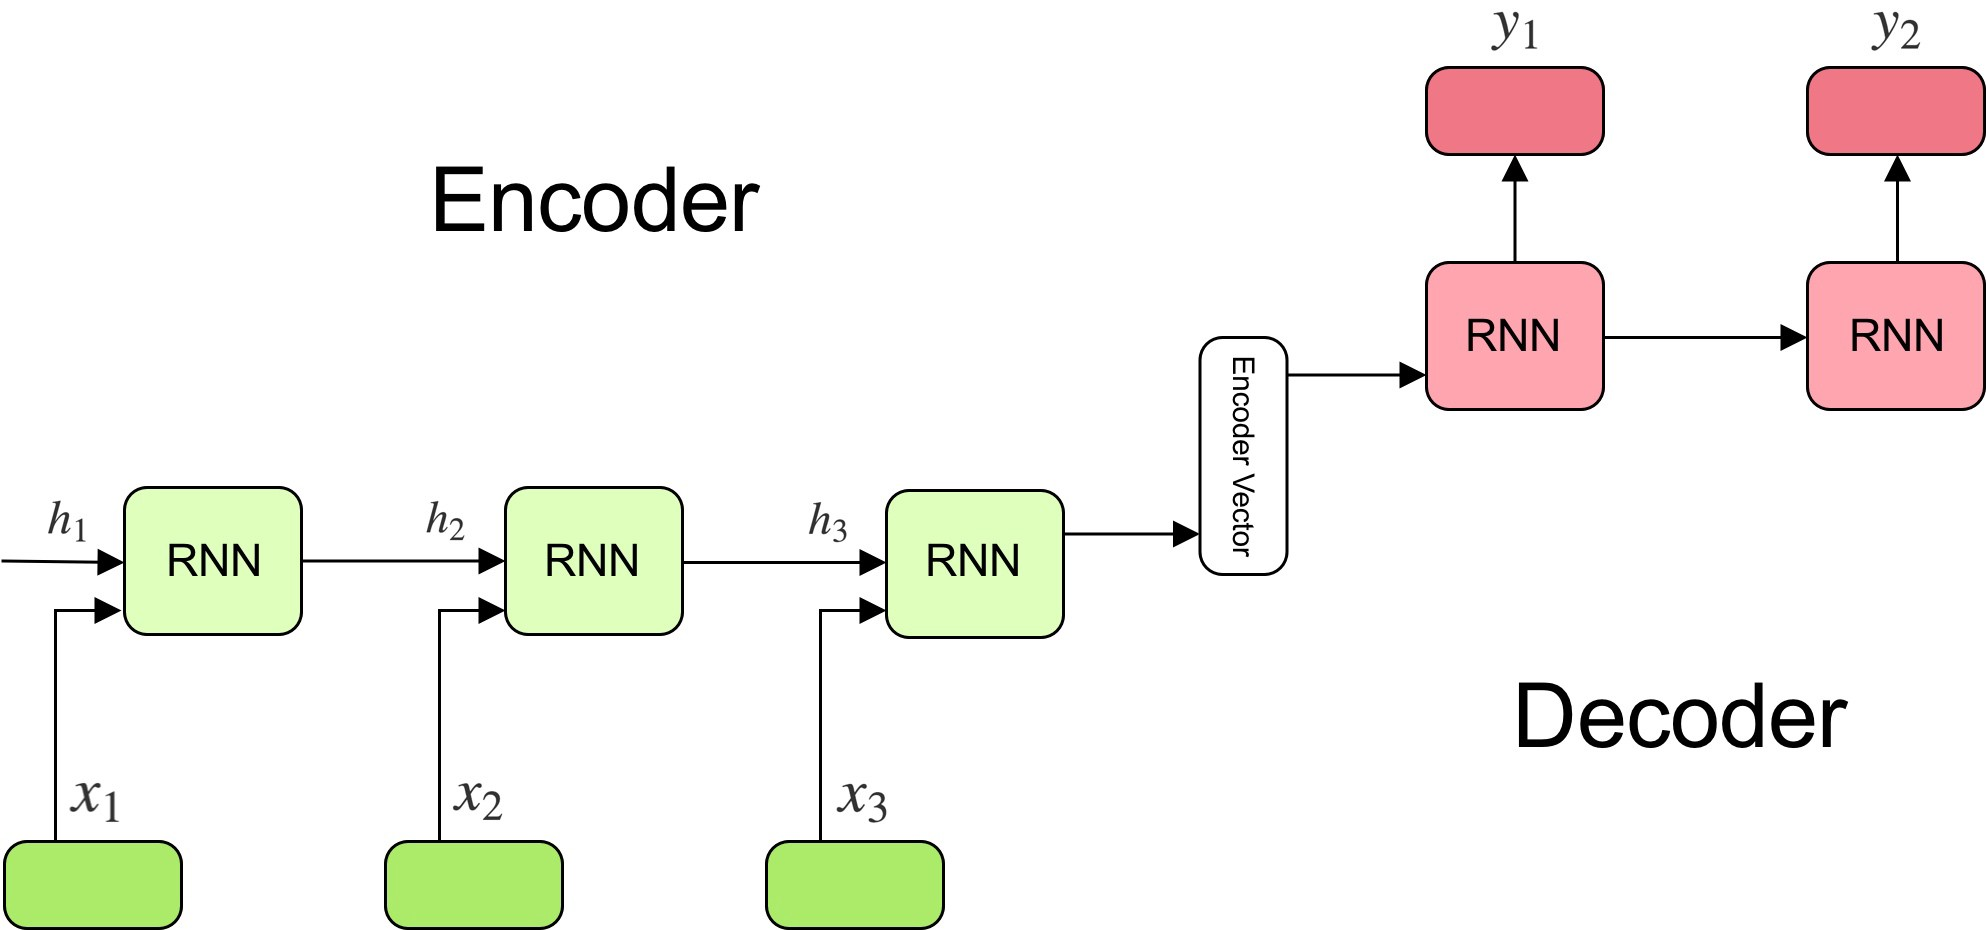
\includegraphics[width=4.5in]{photos/encoderdecoder.jpeg}\\
		\caption{Encoder-decoder sequence to sequence model \cite{encdec}}\label{encdecseq}
	\end{center}
\end{figure}

Figure \ref{encdecseq} shows, that the encoder decoder model is built up from actually three parts:

\begin{itemize}
	\item Encoder
	\item Intermediate (encoder) Vector
	\item Decoder
\end{itemize}


The \textbf{Encoder} iteratively integrates the words in a sentence into the hidden state \textit{h} into the Long Short Term Memory cell.
Figure \ref{lstm3} shows a single LSTM cell with the input cell state \textit{C} at the time step \textit{t-1}  and the input of the hidden state \textit{h} at the same time step \textit{t-1}. This is necessary for the cell to compute both the input words, but also the knowledge from prior words. Words are represented as latent vectors in the sequence to sequence models and are stored in a vocabulary table. Each fixed length vector stands for a word in the vocabulary, for example the vector length is fixed to a dimension of 300. In a simple case, the number of words in the vocabulary is fixed to e.g. 50.000 words, hence the dimension of the vocabulary table in Figure \ref{voctable} is [50000 x 300]. 

\begin{figure}
	\begin{center}
		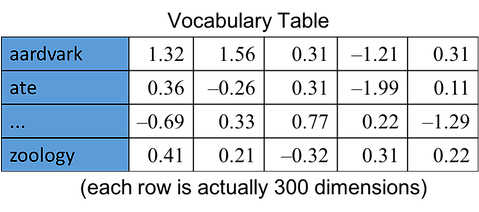
\includegraphics[width=3.5in]{photos/w1-16}\\
		\caption{Snippet of an example vocabulary table \cite{mugan}}\label{voctable}
	\end{center}
\end{figure}

A connection of multiple recurrent units (three in Figure \ref{encdecseq}) where each accept a single element as an input, gains information and propagates it forward to the next cell and accordingly the next time step. In the example of Figure \ref{encdecseq}, the hidden state of \textit{h3} is calculated based on the prior two cells.


The \textbf{Encoder Vector} is the last hidden state of all the encoder cells, in this example the encoder vector is located at the output of cell three. The vector tries to combine all of the information from the prior encoded words with the purpose to help the decoder make accurate predictions. Basically, the encoder vector is the initial input for the decoder part of the model.

The \textbf{Decoder} unrolls the encoder vector from meaning space into a target sentence. The meaning space (shown in Figure \ref{meaningspace}) is a mapping of concepts and ideas that we may want to express to points in a continuous, high-dimensional grid \cite{mugan}. 
The minimum requirement for the meaning space is to consist at least of the last state of the encoder Recurrent Neural Network (encoder vector). The decoder computes a probability distribution for each word in the encoder vector to generate the next state. In the example case, the output is generated by multiplying the hidden state in the encoder vector \textit{h} by the output matrix of size [300 x 50000]. The product of this matrix multiplication is a vector of size [50,000], that can be normalized with a \textit{softmax} into a probability distribution over words in the vocabulary. The network can then choose the word with the highest probability, because the softmax squeeses all outputs into a summed up probability of 1. For example:

\begin{tcolorbox}
	"Since I am living in Hong Kong, by now I speak fluent ... "
	
	\begin{itemize}
		\item Cat: 0.01
		\item running: 0.005
		\item Cantonese: \textbf{0.5}
		\item Mandarin: 0.3
		\item French: 0.015
	\end{itemize}

	The chosen word is \textbf{Cantonese}, because it is the highest probability among all probabilities which are summed up to 100\%
\end{tcolorbox}
 

\subsection{Attention}
In general, the explanation of the sequence to sequence models just covered the very basic idea of the model. To achieve the state-of-the-art result, not only a single vector can be used for encoding the entire input sequence, but multiple vectors each capable of capturing other information. 

\begin{figure}
	\begin{center}
		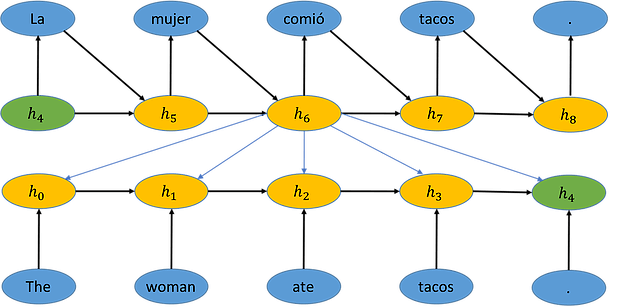
\includegraphics[width=4.5in]{photos/w1-11}\\
		\caption{Attention mechanism for Spanish-English translation \cite{mugan}}\label{attention1}
	\end{center}
\end{figure}
In the encoder and decoder model, the length of the state vector \textit{h} does not change for the input and output. As shown in the example of Section \ref{ss:seq2seq}, sentences translated into another language can have a different word length. For the model to automatically adjust the length of the output, is to use the technology called \textit{attention} \cite{attention} \cite{attention2}.

Figure \ref{attention1} shows the basic concept of attention. The Long Short Term Memory is not starting to right before time step \textit{t = 6} at state \textit{\(h_{6}\)}. Attention enables the network to look at all prior encoded states of the words, takes the weighted average probability of the vectors and also uses this as additional information. Attention also projects its vectors into the meaning space (Figure \ref{meaningspace}. 

\begin{figure}
	\begin{center}
		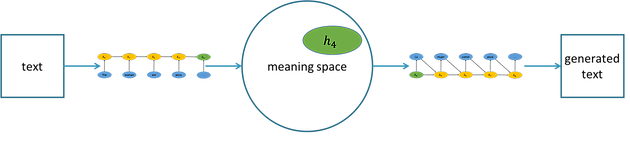
\includegraphics[width=5in]{photos/w1-21}\\
		\caption{Meaning Space of the Attention model \cite{mugan}}\label{meaningspace}
	\end{center}
\end{figure}

Sequence to sequence models can be entirely built up from the attention model \cite{attention2}. 

\section{The Structure of Text Summarization}

In the modern era of big data, retrieving useful information from a large number of textual documents is a challenging task due to the unprecedented growth in the availability of online blogs, forums, news, and scientific reports that are tremendous. Automatic text summarization provides an effective and convenient solution for reducing the amount of time it takes to read all the information. The goal of text summarization is to compress long documents into shorter summaries while maintaining the most important information and semantic of the documents \cite{ts-intro} \cite{ts-intro2}. Having the short summaries, the text content can be retrieved, processed and digested effectively and efficiently. 
Generally speaking, there are two basic approaches for performing a text summarization: Extractive and Abstractive \cite{ts-intro3}. 

As mention from the Section \ref{ss:history}, there is a text-to-text and data-to-text approach. The text-to-text method is mostly used in the context where a single document is the only input for generating the text. It can be seen as an extractive approach.  On the other side the abstractive approach is actually a data-to-text methods, because it takes into account multiple inputs, such as the text, opinion or another vocabulary.

Jones et al. in 1999 defined and classified text summarization by the following three summarization factors \cite{Jones98automaticsummarising:} (Pages 1-12):

\begin{itemize}
	\item \textbf{Input}: single and multi document
	\item \textbf{Purpose}: informative and indicative
	\item \textbf{Output}: extractive and abstractive
\end{itemize}

This three factors will be explained in the following.

\begin{figure}
	\begin{center}
		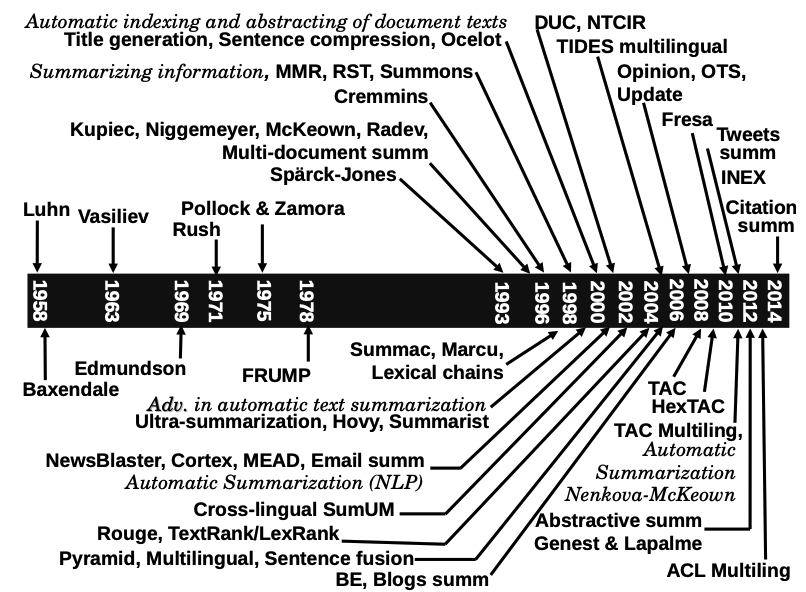
\includegraphics[width=5.5in]{photos/history}\\
		\caption{Highlights of automatic text summarization \cite{juan} (Page 17)}\label{hist}
	\end{center}
\end{figure}

Even though I cannot explain the single state of the art steps at each time in Figure \ref{hist}, I think it provides an good overview on the development of automatic text summarization. Everything started with Peter Luhn from Germany in 1958.

\subsection{Input}\label{ss:input}

The input has two crucial variables, that can change the way how to process the summary completely. The input variable denotes whether the input comes from a \textbf{single-document} or from a \textbf{multi-document}. 

\subsubsection{Single-Document}\label{ss:sd}
The most simple task for an automized summarization system is a generic single document summary. This was first introduced by Peter Luhn's work in 1958, an extractive method to summarize a text \cite{textmining1958}.  Even though this first approach was first proposed over 60 years ago, it is still not completely solved. The pipeline for a single document summary is as follows \cite{juan} (Page 69):

\begin{itemize}
	\item \textit{Preprocessing}: Split sentences into words, cut stopwords (and, that, there, ..) out and filter out punctuation 
	\item \textit{Extraction}: Calculate and combine similarity measure between words and/or sentences, sort and select the sentences
	\item \textit{Generarion}: Assemble, postprocess and reformulate extracted sentences
\end{itemize}

\begin{figure}
	\begin{center}
		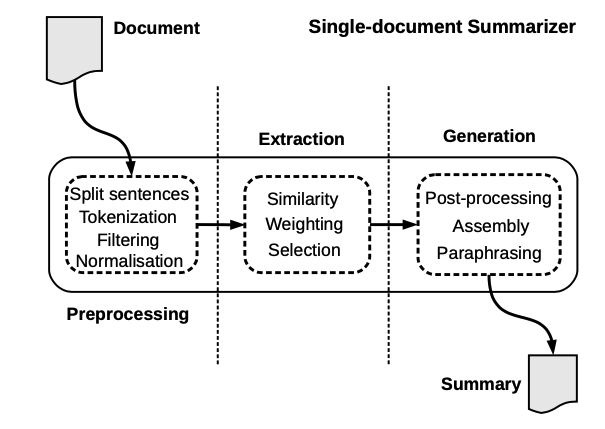
\includegraphics[width=4.5in]{photos/single_doc}\\
		\caption{General architecture of a extraction-based single-document summarization system \cite{juan} (Page 70)}\label{single}
	\end{center}
\end{figure}

Figure \ref{single} shows a standardized pipeline, also called \textit{Natural Language Processing Pipeline}. For measuring the similarity between words and sentences, several methods are possible to achieve this goal. It would exceed this thesis if I explain all different methods, but I still want to mention them, because it is the core part of the original pipeline middle-step:

\begin{itemize}
	\item Latent Semantic Analysis (LSA)
	\item Graph-based approaches
	\item Statistical metrics
\end{itemize}

The \textbf{Latent Semantic Analysis} \cite{Deerwester90indexingby} is a model which allows semantics to be represented from the following ideas: two words are semantically close if they appear in similar contexts and two contexts are similar if they contain semantically close words. The words in a (large) corpus are represented in the occurrence matrix S. The matrix S stores, for every single word in the corpus, the contexts in which the words appeared and additionally also their appearance frequency \cite{juan} (Page 73). This technique measure therefore relationships between different words. After finishing this process, the Latent Semantic Analysis assumes accordingly that words close in meaning occur in similar pieces of text.

\textbf{Graph-based approaches} conduct to represent content of textual information from single documents. There are countless variations of graph-based approaches and I have already used one so far. In Section \ref{ss:ref} for the Box \ref{box:1}, the part-of-the-speech tagging is a method in the graph-based approaches. In general, the vertices or nodes are assimilated to semantic collections of words and sentences and the edges of the nodes represent the relations between each words and collections. 
Another widely used approach is \textit{bag-of-word}. I used that as an example in Section \ref{ss:data} for Figure \ref{corpus}. Different unique words are packed together into a corpus and each occurrence of the word is counted and summed together. The ANK algorithm from Lawrence Page in 1998 \cite{brin1998anatomy} (Pages 107-118) paved the way for the success in web page retrieval (scraping): web pages are ranked by their popularity in the network (how often each page is clicked by users), rather than by the amount or quality of their content. This type of algorithm computes the importance of the vertex of the graph, based on the general information gathered from a recursive analysis of the complete graph, rather than a local analysis of a vertex \cite{juan} (Page 77).

\subsubsection{Multi-Document}\label{ss:multi}

Multi-document summarization faces different problems than the single-document summarization. The sentence extraction methods (Latent Semantic Analysis and graph-based approaches) can also be applied to multi-document summarization. The problem of redundancy in the documents is can be always present in multi-document summarization. The typically does not happen in the single-document case. Redundancy has a huge impact on the coherence and the cohesion of this new type of extract \cite{juan} (Page 109). Multi-document summarization is basically the extension of single document summarization, but like already said, redundancy is not the only issue. The basic pipeline is shown in Figure \ref{multi}. 

\begin{figure}
	\begin{center}
		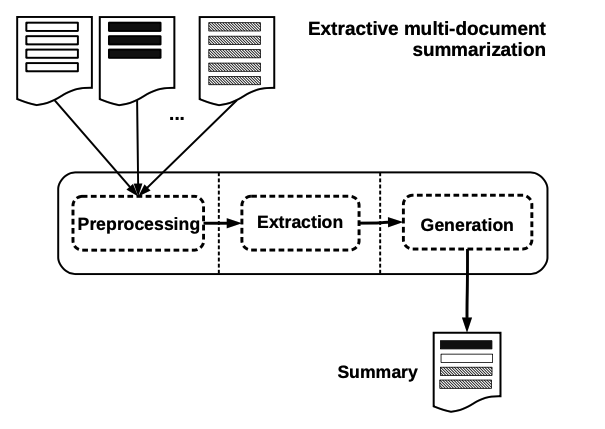
\includegraphics[width=4.5in]{photos/multidoc}\\
		\caption{Extraction based multidocument summarization system \cite{juan} (Page 110)}\label{multi}
	\end{center}
\end{figure}

Multi-document input are likely to have the same or a similar topic, but it is not necessary. The first automation system was developed by McKeown and Radev in 1995 until 1998 \cite{radev-mckeown-1998-generating} (Pages 469-500). My case study example Google News is a typical example for multi-document summarization, because Google multiple sources of information (scrape news from different other websites), collect the information and process them through the pipeline (Figure \ref{multi}). The key task is therefore not only detecting and eliminating redundancy, but also notice novelty and ensure that the generated summary is coherent and without missing points \cite{Das07asurvey} (Page 11).
 
The input for the summarization system are multiple documents such as \(D_{1}, D_{2},..., D_{n}\), where \textit{D} is single document and \textit{n} is the total number of single-document, combined into a multi-document input.
The preprocessing step in the multi-document summarization is quite similar, but the same as in the single-document summarization. The four steps for the multi-document are:
 
\begin{itemize}
	\item \textbf{Sentence segmentation}: Each document \textit{D} is segmented for itself as \(D = {S_{1}, S_{2},..., S_{m}}\), where every \textit{S} denotes a single sentence in document \textit{D}. The number of sentences is denoted as \textit{m}.
	\item \textbf{Tokenization}: Words of each sentence \textit{S} are tokenized into \(T = {t_{1}, t_{2},..., t_{k}}\) \textit{k} terms \textit{t}, where every \textit{t} represents a distinct term occurring in \textit{D}. 
	\item \textbf{Stop word removal}: The most commonly used words in every language are stored in a so-called stop-word-table. Words from that table occurring in a document \textit{D} are removed. Example words are 'a', 'an' or 'the'. As already mentioned in the single-document summarization
	\item \textbf{Stemming}: converts words back into the base form. For example (houses -> house, running -> run). This is done to avoid redundancy.
\end{itemize}
 
 
After preprocessing the documents into word form, weights are computed to get a sentence informative score. This score is calculated for every sentence accordingly and is used as the input for a chosen optimization algorithm. This happens in the \textit{Extraction} box of Figure \ref{multi}. Like for the single-document, there are multiple methods to calculate extraction weights:

\begin{itemize}
	\item Abstraction and Information Fusion
	\item Topic-driven summarization
	\item Graph Spreading Activation
\end{itemize}

\textbf{Abstraction and Information Fusion} contains basically of two steps. At first, like in the most methods, a similarity measurement on word or sentence level is computed. When using an abstractive approach (Section \ref{ss:exabs}), the TFIDF score is commonly used. TFIDF is an information retrieval technique that weighs a term’s frequency (TF) and its inverse document frequency (IDF). Every term has its respective TF and IDF score. The product of the TF and IDF scores of a term is called the TFIDF weight of that term \cite{Ramos_usingtf-idf}. For each term, a vector is calculated that represents matches on the different features. Decision rules that were trained and learned from the data are used to classify each pair of text as either similar or dissimilar. This further feeds a subsequent algorithm that imputes the most related terms in the same topic-theme \cite{Das07asurvey} (Page 13). Once this scores and vectors are computed, the second step \textit{information fusion} starts. This step decides which information should be used for generating the final summary. Rather than just selecting a sentence that holds as a group representative, an algorithm which compares predicated argument structures of the terms. Within each topic, the algorithm needs to determine which terms are used and repeated often enough to be included into the summary.

\textbf{Topic-driven summarization} techniques aim to detect words that describe the topic of the multiple input documents. An advance of the initial idea of Luhn (proposed in Section \ref{ss:sd}) was to use the log-likelihood ratio test to identify special words known as the \textit{topic signatures} \cite{textmining1958}. The log-likelihood is often used in statistical approaches for the text summarization. 
There are two ways to calculate the importance of a sentence. First, as a function which contains the number of its topic signatures, or as the proportion of all the topic signatures in each sentence respectively. While the first method gives usually higher scores to longer sentences, the second approach measures the occurrences of the topic words \cite{dunning-1993-accurate}.

\textbf{Graph Spreading Activation} is a similar approach than the graph-based approach from the single-document summarization. The PAGERANK algorithm can be used for this approach, or other alternations like LexRank and TextRank. 


\subsection{Purpose}

\textbf{Types of Summaries}

The \textit{informative summary} contains the informative part of the original text. The main ideas from the text should be transmitted, for example the abstract of research articles, where authors try to present the essential core of the reasearch, is an informative summary. Whereas an indicative summary tries to transmit the relevant contents of the original document in such a way, so that the readers can chose documents that match with their interests to read further.

An \textit{indicative summary} is not meant to be a substitute for the original document. The opposite is the informative summary, which can replace the original documents as far as the important contents is concerned and by how much it was shortened down.

The \textit{keyword summary} tries to summarize the text into only keywords. Words will be weighted by their importance and the most crucial ones are selected without caring for the grammar.

The \textit{headline summary} is the type of summary from the case study in Section \ref{ss:case}. The entire text gets compressed into a single sentence. It is a single line summary.

\textbf{Generic vs. user-oriented}

Generic systems generate summaries that consider all of the given information from the documents. On the other hand try user-oriented systems to produce personalized summaries that concentrate on specific information from the original documents. Like News could only summarize the conservative or right-wing news, if someone only searches for right-wing content.

\textbf{General purpose vs. domain-specific}

General-purpose summarizers can be used across any domains with barely no modification needed. In contrary, domain-specific systems are programmed to process documents for a specific domain, like the research, news or book summarizing domain.

\subsection{Output}\label{ss:exabs}

During this thesis I have already mentioned the two core differences between text summarization. The extractive and abstractive approach. I use the definition of See et al. from 2017, where he regards the extractive summarizer as an explicit selection method for text snippets inside the single- or multi-document. While the abstractive summarizer generates novel text snippets to describe summaries from a higher point of view by using vocabulary not included in the source input \cite{see-etal-2017-get} (Pages 1073-1083). 

\begin{figure}
	\begin{center}
		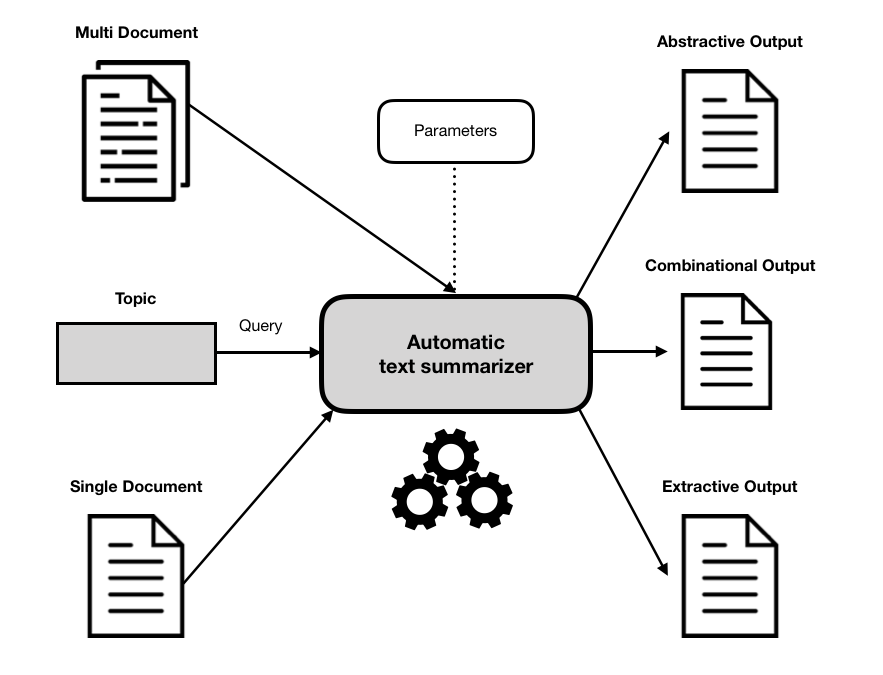
\includegraphics[width=5in]{photos/abex}\\
		\caption{Simplified Abstraction Extraction process}\label{abex}
	\end{center}
\end{figure}

Figure \ref{abex} shows the general model pipeline for either the extractive or abstractive approach. There is also a relatively new combinational approach, which will be explained in Section \ref{ss:trends} (\textit{Advanced Approaches for Text Summarization}). The topic input into the automatic text summarizer has already been explained in the multi-document Section \ref{ss:multi}. The parameter input contains for example the compression rate \(\tau\). This could a a value like 15\%, which means that the length of the original input document will be reduced by 85\%.

\subsubsection{Extractive}
	
The aim of the extractive approach is to give an overview about the source document. This is done by selection fragments of the text (words, sentences or paragraphs) that contain the essential information of the input text or texts. It can be seen as an copy and paste action for the most important fragments. Figure \ref{extract} shows the basic structure of an extractive summarizer, where the selection part is one of the three categorical types. The extractive approach has still some valid use cases, because:

\begin{itemize}
	\item \textbf{Pros}: The approach is robust, because it uses existing natural-language phrases that are taken directly from the input.
	\item \textbf{Cons}: It lacks in flexibility since it cannot use novel words or connectors. Furthermore it cannot paraphrase like a human could do it. Sometimes the approach even applied wrong grammar.
\end{itemize}

According to Radev et av. in the 2002, extractive text summarization can be categorized as three different types \cite{ts-intro} (Pages 399-408):

\begin{itemize}
	\item Surface-level
	\item Intermediate-level
	\item Deep parsing techniques
\end{itemize}

\begin{figure}
	\begin{center}
		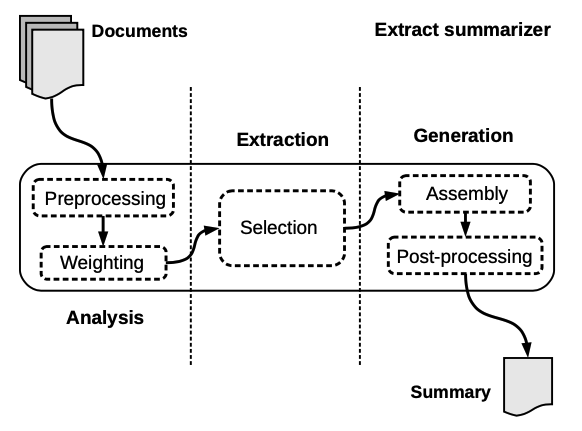
\includegraphics[width=4in]{photos/extract}\\
		\caption{General architecture of an extraction-based summarization system \cite{juan} (Page 31)}\label{extract}
	\end{center}
\end{figure}


The \textbf{surface-level} algorithms scratches on the linguistic easy understandable parts on the text. It cannot detect deep connections and abstractive features. It rather uses certain linguistic elements to detect the most important segments of a document \cite{juan} (Page 32). The mentioned inventor of automatic text summarizer Luhn \cite{textmining1958} used a surface-level techniques weight the occurrences of words in sentences. This technique is good for headline or keyword summarization. 

The \textbf{intermediate-level} categorization digs deeper into the meaning of certain paragraphs. It uses linguistic information to find relations between lexical semantic sequences. This approach is more appropriate for extractive text summary than the surface-level approach.

The \textbf{deep parsing techniques} approaches make use of deep linguistic techniques that exploit the discursive structure of the input document or documents. It can find good relations in the text and one of the earliest methods was published by Marcu in the year 2002 \cite{marcu}. He split the text into discursive units and uses a minimal set of relations, called discourse segmentation. An algorithm weights and orders the elements accordingly. The highest weighted elements will be selected for the summary.

Even though I proposed in the Section \ref{ss:input} for the single-document and multi-document different methods to compute the weights for the words, the extractive approach and the abstractive approach can be applied for both single- and multi-documents. The most common methods for the extractive approach to calculate weights are:

\begin{itemize}
	\item Graph-based (both single-document and multi-document) like PAGERANK and Textrank
	\item Luhn's algorithm \cite{textmining1958}, 
	\item Topic-driven (Section \ref{ss:multi}) 
	\item Neural Network approach (Section \ref{ss:neuralgen} - \textit{Advanced Approaches for Text Summarization})
\end{itemize}

\subsubsection{Abstractive}

\subsection{Evaluation}\label{ss:ev}



\section{Advanced Approaches for Text Summarization}\label{ss:trends}

\subsection{Neural Text Summarization}\label{ss:neuralgen}

\begin{figure}
	\begin{center}
		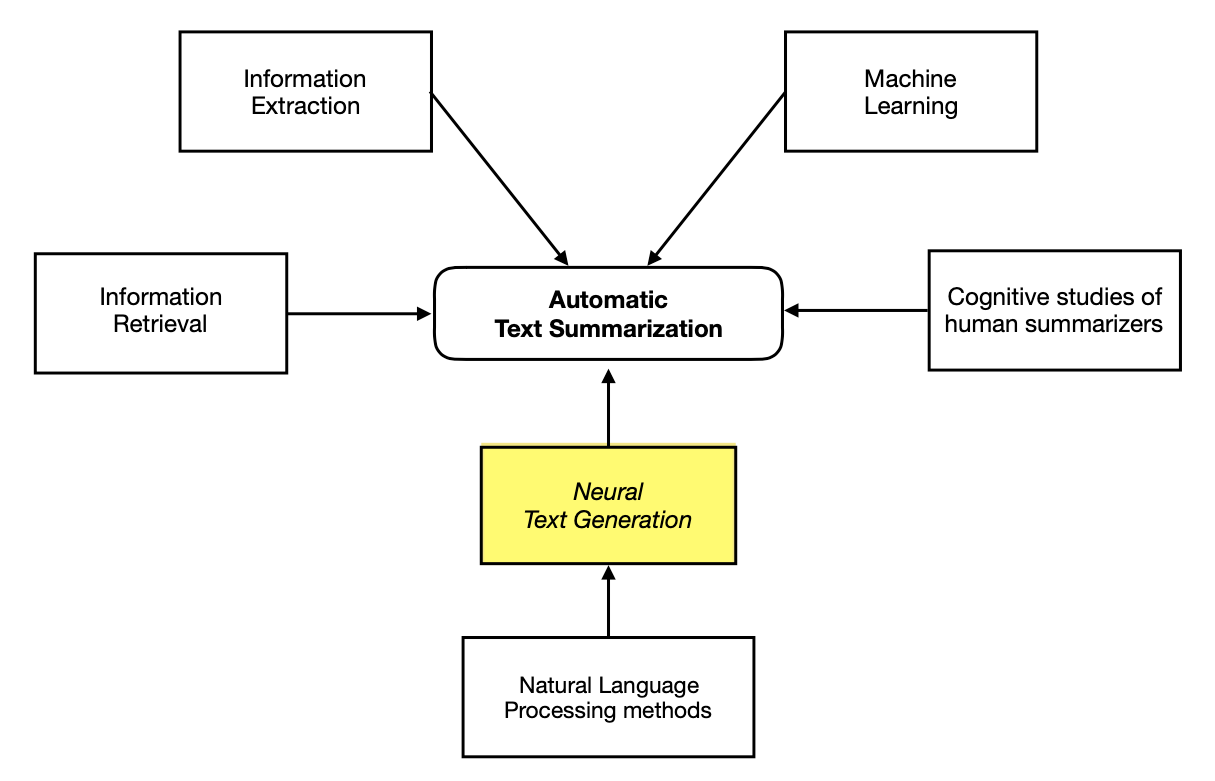
\includegraphics[width=5.5in]{photos/summ}\\
		\caption{Research fields with influence on the development of text summarization}\label{summ}
	\end{center}
\end{figure}

\subsection{Combinational Approach}

\subsection{Reinforcement Learning}
